\documentclass [11pt, a4wide, twoside]{article}

\usepackage{times}
\usepackage{epsfig}
\usepackage{ifthen}
\usepackage{xspace}
\usepackage{fancyhdr}
\usepackage{moreverb}
\usepackage{amsmath}
\usepackage{url}

% solution switch
\newboolean{showsolution}
\setboolean{showsolution}{true}
\setboolean{showsolution}{false}



%layout
\topmargin      -5.0mm
\oddsidemargin  6.0mm
\evensidemargin -6.0mm
\textheight 215.5mm
\textwidth      160.0mm
\parindent        1.0em
\headsep          10.3mm
\headheight        12pt
\lineskip    1pt
\normallineskip     1pt

%header
\lhead{Programming Languages \\ 2021}

\rhead{Prof. O. Nierstrasz\\
Mohammadreza Hazhirpasand, Joel Niklaus}
\lfoot{page \thepage}
\rfoot{\today}
\cfoot{}

\renewcommand{\headrulewidth}{0.1pt}
\renewcommand{\footrulewidth}{0.1pt}

\renewcommand{\thesubsection}{\arabic{subsection}}

%enumeration
\newenvironment{myitemize}{%
     \begin{itemize}
     \setlength{\itemsep}{0cm}}
     {\end{itemize}}

\newenvironment{myenumerate}{%
     \begin{enumerate} \setlength{\itemsep}{0cm}}
     {\end{enumerate}}


%solution
\ifthenelse{\boolean{showsolution}}
   {  \newcommand{\solution}[1]{
   	\noindent\underline{\textbf{Answer:}}\\[2mm]
   	 \textsl{#1}
	 \vspace{10pt}
	 \normalsize
	}
  }
  {  \newcommand{\solution}[1]{} }

\newcounter{exnum}
\def\xexercise{\fontsize{12}{10}\fontseries{bx}\selectfont}
\def\xnormal{\fontseries{m}\fontshape{n}\selectfont}


\newcommand{\exercise}[1]{%
     {\addtocounter{exnum}{1}\vskip 0.8cm{\xexercise \noindent Exercise
\arabic{exnum} (#1)} \xnormal} \vskip 0.3cm} 
 \newcommand{\aufgabe}[1]{
     {\addtocounter{exnum}{1}\vskip 0.8cm{\xexercise \noindent Aufgabe
\arabic{exnum} (#1)} \xnormal} \vskip 0.3cm} 

\pagestyle{fancy}


% ===============ABBREVIATIONS==============================
\newcommand{\eg}{\emph{e.g.,}\xspace}
\newcommand{\ie}{\emph{i.e.,}\xspace}
\newcommand{\etc}{\emph{etc.}\xspace}


\begin{document}

% title
\section*{
    \ifthenelse{\boolean{showsolution}}{Solution }{}
    \xspace{}Serie 8 - Objects and Prototypes}

%==============================================================================
%\subsection{Notes}
JS Material and tutorials: \\ \\
%\url{http://scg.unibe.ch/download/lectures/pl/}\\
%and\\
\url{http://scg.unibe.ch/teaching/pl/resources}\\ \\
% Pass by my office for more material.

%==============================================================================
\subsection{Theoretical Questions}

\begin{myenumerate}

\item What happen if we assign a variable without using the command ``var''? Which problems could cause?

\solution{the variable is created on the fly and it will have global scope so it will override the value of a global variable with the same name.}


\item How do you extend all objects created with a specific constructor?

\solution{With the mechanism of prototype. }


\item What is a closure?

\solution{Inner functions are closures.}


%\item How would you implement private static properties?
%
%\solution{By using closures for the methods and properties of an object.}


\item What is the difference between delegation and inheritance?

\solution{}


\item How would you access arguments of a function with variable number of arguments? 

% \solution{
% \begin{verbatim}
% function printall() {
% 	for (var i = 1; i < arguments.length; i++)	 
% 		console.log(arguments[i])
% }
% \end{verbatim}
% }


\end{myenumerate}



%%==============================================================================
%\subsection{Events}
%
%Build a HTML page where the function in snippet below triggers or can be triggered: when I open the page, when I press a button, when I click with the mouse, when I double click with the mouse, when I go with the mouse over an area, when I move the mouse out of an area, when I press the mouse left button and when I release the mouse left button.
%
%\begin{verbatim}
%<script type="text/javascript">
%
%function helloworld() {
%  alert("Hello world");
%}
%</script>
%\end{verbatim}
%
%\solution{\begin{verbatim}
<!DOCTYPE HTML PUBLIC "-//W3C//DTD HTML 4.0 Transitional//EN">
<html>
<head>
<title>Corso JavaScript ad esempi</title>

<script type="text/javascript">

function helloworld() {
  alert("Hello world");
}
</script>

</head>

<body onLoad="helloworld();" onKeyUp="helloworld();">

<h2> Mouse Events</h2>
<a href="#" onClick="helloworld();">click</a> <br/><br/>
<a href="#" onDblClick="helloworld();">Double click</a> <br/><br/>
<a href="#" onMouseDown="helloworld();">Mouse Down</a> <br/><br/>
<a href="#" onMouseUp="helloworld();">Mouse Up</a> <br/><br/>
<a href="#" onMouseOver="helloworld();">Mouse Over</a> <br/><br/>
<a href="#" onMouseOut="helloworld();">Mouse Out</a> <br/><br/>

</body>
</html>
\end{verbatim}

}


%==============================================================================
\subsection{Poor Platypus}

A possible classification for animals is the one shown in Figure \ref{fig:ex2}. When it comes to classify the platypus you realize that it nurses but it also spawns. So implement the class diagram shown in figure \ref{fig:ex2} including the poor platypus in Java Script. Use the ex2/poorPlatypusToSolve.html file as skeleton for your implementation. 

\begin{figure}[ht!]
\begin{center}
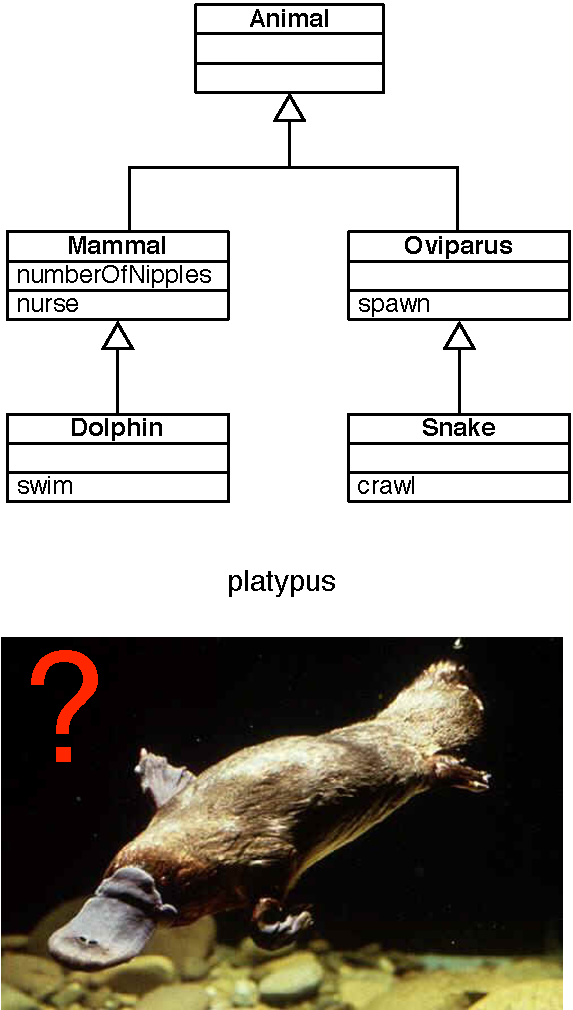
\includegraphics[width=0.4\columnwidth]{ex2/Ex2.pdf}
\caption{Animal classification}
\label{fig:ex2}
\end{center}
\end{figure}

\solution{\begin{verbatim}
<html>
<head>
<title>Platypus</title>
<script type="text/javascript">

var animal = {}

var mammal = Object.create(animal);
mammal.numberofNipples = 2;
mammal.nurse = function () {
	alert("I am nursing");
}
mammal.getNumberOfNipples = function(){
	alert(this.numberofNipples);
}

dolphin = Object.create(mammal);
dolphin.numberofNipples = 4;
dolphin.swim = function() {
	alert("I am swimming");
}

var oviparus = Object.create(animal);
oviparus.spawn = function() {
	alert("I am spawning");
}

var snake = Object.create(oviparus);
snake.crawl = function() {
	alert("I am crawling");
}

var platypus = Object.create(mammal);
platypus.numberofNipples = 6;
platypus.spawn = oviparus.spawn;

function display(text) {
	document.getElementById("output").innerHTML += text + "\n";
}

</script>
</head>
<body>
<pre id="output">
</pre>
<a href="#" onClick="mammal.getNumberOfNipples();">mammal's number of nipples</a> <br/><br/>

<a href="#" onClick="dolphin.swim();">dolphin swimming</a> <br/><br/>
<a href="#" onClick="dolphin.nurse();">dolphin's nursing</a> <br/><br/>
<a href="#" onClick="dolphin.getNumberOfNipples();">dolphin number of nipples</a> <br/><br/>


<a href="#" onClick="snake.crawl();">snake crawling</a> <br/><br/>
<a href="#" onClick="snake.spawn();">snake spawning</a> <br/><br/>

<a href="#" onClick="platypus.nurse();">platypus nursing</a> <br/><br/>
<a href="#" onClick="platypus.spawn();">platypus spawning</a> <br/><br/>
<a href="#" onClick="platypus.getNumberOfNipples();">platypus's number of nipples</a> <br/><br/>
</body>
</html>
\end{verbatim}

}


% ==============================================================================
\subsection{Post Office}

Some public places nowadays have special rules so to serve high priority customers first independently from when they entered the queue. Simulate in Java Script a post office where high priority customers are served first. Use the ex3/postofficeToSolve.html file as skeleton for your implementation.

\solution{\begin{verbatim}
<html>
<head>
<title>Post Office</title>
<script type="text/javascript">
// Sample solution; Oscar Nierstrasz 2012.05.02
var customer = {
	name : '(unknown)',
	priority : function() {
		return false;
	},
	// Hint: define toString() to make an object printable 
	toString : function() {
		return this.name;
	}
}

var bob = Object.create(customer);
bob.name = 'Bob';
var carol = Object.create(customer);
carol.name = 'Carol';
var ted = Object.create(customer);
ted.name = 'Ted';
var alice = Object.create(customer);
alice.name = 'Alice';

var special = Object.create(customer);
special.priority = function() {
	return true;
}
var ray = Object.create(special);
ray.name = 'Ray';
var ludwig = Object.create(special);
ludwig.name = 'Ludwig';

// Hint: use JavaScript arrays to represent queues.
var customers = [ bob, carol, ray, ted, ludwig, alice ];

// Hint: make Post Office a closure
var postoffice = (function() {
	var queue = [];
	var counter = [ [], [] ];
	var enterCustomer = function() {
		if (customers.length > 0) {
			var newCustomer = customers.shift();
			if (newCustomer.priority()) {
				queue.unshift(newCustomer);
			} else {
				queue.push(newCustomer);
			}
		}
		updateQueue();
	}
	var updateQueue = function() {
		updateCounter(1);
		updateCounter(2);
		updateDisplay();
	}
	var updateCounter = function(n) {
		if (queue.length > 0) {
			if (counter[n-1].length == 0) {
				counter[n-1].push(queue.shift());
			}
		}
	}
	var updateDisplay = function() {
		// Hint: use Array.join() to concatenate array elements
		show('queue', queue.join(', '));
		show('counter1', counter[0].join(', '));
		show('counter2', counter[1].join(', '));
	}
	var serve = function(n) {
		if (counter[n-1].length > 0) {
			customers.push(counter[n-1].shift());
		}
		updateQueue();
	}
	return {
		enterCustomer : enterCustomer,
		serve : serve
	}
})();

function show(id, text) {
	document.getElementById(id).innerHTML = text;
}
</script>
<style>
table, th, td {
	border: 1px solid black;
}
</style>
</head>
<body>
<h1>Post Office</h1>
<p>Bob, Carol, Ted and Alice are regular customers. Ray and Ludwig are special customers with priority service, and always go to the head of the queue.</p>
<table>
	<tr>
		<td><strong>Queue</strong></td>
		<td id="queue"></td>
	</tr>
	<tr>
		<td><strong>Counter 1</strong></td>
		<td id="counter1"></td>
	</tr>
	<tr>
		<td><strong>Counter 2</strong></td>
		<td id="counter2"></td>
	</tr>
</table>
<button type="button" onclick="postoffice.enterCustomer()">Customer enters</button>
<button type="button" onclick="postoffice.serve(1)">Serve counter 1</button>
<button type="button" onclick="postoffice.serve(2)">Serve counter 2</button>

</body>
</html> 
\end{verbatim}
}


\end{document}

